% Name: Simple pendulum
% Description: A bob on a string at angle θ from the vertical, with the tension, its weight, the weight's parts along and across its path, and the arc it swings on.
% Tags: pendulum, oscillation, forces, small angles

\usetikzlibrary{arrows.meta, angles, quotes, patterns}

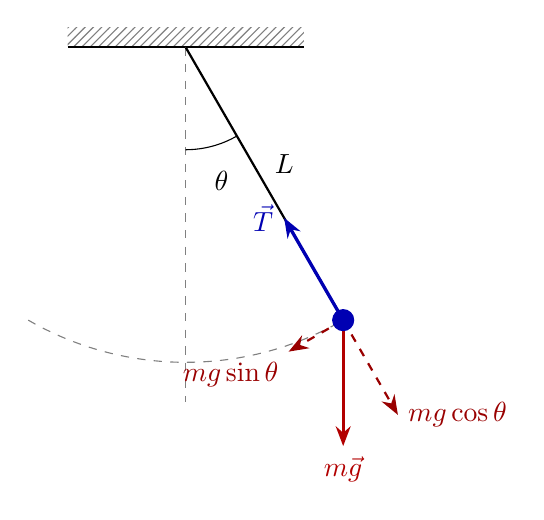
\begin{tikzpicture}[>={Stealth[length=2.5mm]}, force/.style={->, very thick}]
  \fill[pattern=north east lines, pattern color=gray] (-1.5,0) rectangle (1.5,0.25);
  \draw[thick] (-1.5,0) -- (1.5,0);
  \coordinate (O) at (0,0);
  \coordinate (D) at (0,-4);
  \coordinate (B) at (-60:4);
  \draw[dashed, gray] (O) -- (0,-4.5);
  \draw[dashed, gray] (-120:4) arc[start angle=-120, end angle=-60, radius=4];
  \pic[draw, "$\theta$", angle eccentricity=1.35, angle radius=13mm] {angle = D--O--B};
  \draw[thick] (O) -- node[above right] {$L$} (B);
  % Weight 1.6 down; along the path 0.8 (sin 30), across it 1.39 (cos 30).
  \draw[force, blue!70!black] (B) -- ++(120:1.5) node[left] {$\vec{T}$};
  \draw[force, red!70!black] (B) -- ++(0,-1.6) node[below] {$m\vec{g}$};
  \draw[->, thick, dashed, red!60!black] (B) -- ++(-150:0.8) node[below left] {$mg\sin\theta$};
  \draw[->, thick, dashed, red!60!black] (B) -- ++(-60:1.39) node[right] {$mg\cos\theta$};
  \fill[blue!70!black] (B) circle (4pt);
\end{tikzpicture}
